\section{Future development}
\label{sec:future}

This chapter will develop several idea that could be implemented in future development of POP-C++ VS. 

\subsection{Pseudo Main Node}
As explained in Chapter \ref{sec:security}, the node running the main of a POP-C++ application is exposed to some risks. To avoid to use the developer node or an Admin VM as the Main Node, a mechanism of pseudo Main Node could be developed. \s

The pseudo Main Node should be a VM running POP-C++ Secure and started by the Admin VM. Figure \ref{fig:pseudomain} shows a schematic view od a ESXi Node running POP-C++ VS and a VM acting as a pseudo Main Node. This mechanism should work as follows:

\begin{enumerate}
\item An application is started on the Admin VM.
\item The Admin VM dected the start of an application, starts the Pseudo Main Node VM and transfer necessary information on this VM. The application is then started from this VM. 
\item The Pseudo Main Node asks for resources to the Admin VM. 
\item The Admin VM starts a worker to give resources to the application.
\end{enumerate}


\begin{figure}[ht]
	\caption{Schematic view of the an ESXi Node with "Pseudo Main Node VM"}
  	\centering
	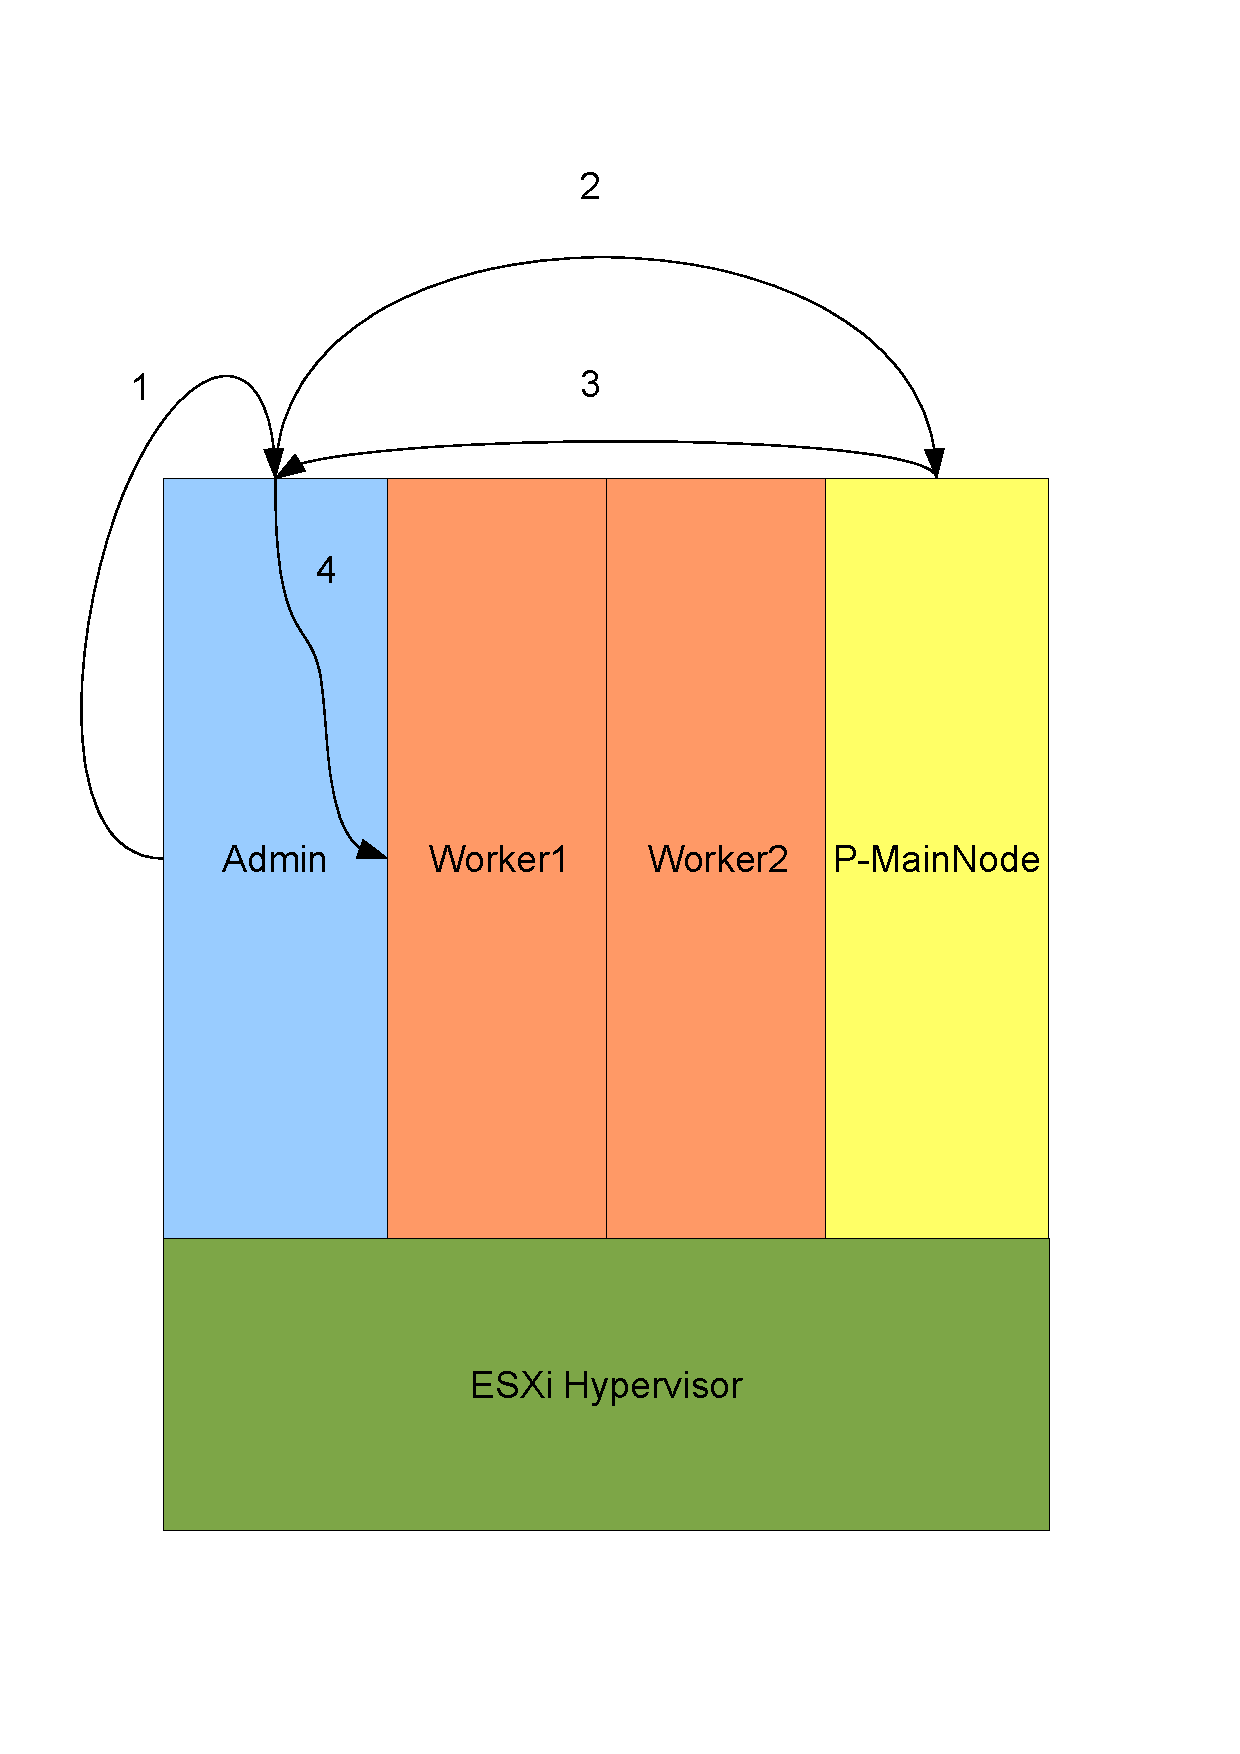
\includegraphics[width=0.5\textwidth]{./pic/pseudomain.pdf}
	\label{fig:pseudomain}
\end{figure}

These steps could be performed by the \textbf{popcrun} script or by the paroc\_main function. 

\subsection{Lock Worker VM}
As Worker VM will execute unknown executable, it could be a great idea to lock as much as possible the outgoing traffic on this VM. On Ubuntu distribution, a simple command line utility named "ufw" allows to apply rules for outgoing and incoming traffic.



\subsection{Keep keys table for each workers}
At the moment, each time a key need to be rerouted, it's done. What could be a great enhancement is to keep a table in the JobMgr about each workers and the keys that have been written on this worker. With this kind of table, we will be able to know if a key has to be wrriten on the worker or not. 